% =============================================================================
% CAPÍTULO 2 - BLOQUE 2.3: ESTUDIO PROFUNDO DE GOOGLE GEMINI EMBEDDING 2:
% ARQUITECTURA OMNIMODAL, MODOS DE INGESTIÓN, MODELADO DE CUOTAS Y RESILIENCIA
% =============================================================================

\subsection{Estudio Profundo de Google Gemini Embedding 2}
\label{subsec:gemini_embedding_2}

\subsubsection{Arquitectura Omnimodal Unificada y Configuración del Espacio de Salida}
\label{subsubsec:arquitectura_gemini_embedding_2}

Dentro de la macrotendencia de modelos fundacionales propietarios accesibles mediante interfaz de programación de aplicaciones (API), \textbf{Gemini Embedding 2} (identificado técnicamente en el catálogo de desarrollo como \texttt{gemini-embedding-2-preview}) constituye el hito arquitectónico de Google hacia la vectorización omnimodal nativa \cite{gemini_emb2_docs, gemini_embeddings_general_docs}. %[cite: 3, 4]
A diferencia de las arquitecturas multimodales de primera generación que requerían codificadores separados y proyecciones post-hoc para cada tipo de dato, \texttt{gemini-embedding-2-preview} ha sido entrenado de extremo a extremo para ingerir texto libre, imágenes estáticas, secuencias de vídeo, pistas de audio y documentos estructurados (archivos PDF) proyectándolos directamente en un único espacio vectorial continuo \cite{gemini_emb2_docs, openrouter_gemini_emb2}. %[cite: 3, 4, 5]

Esta unificación topológica implica que los vectores generados a partir de una consulta textual en lenguaje natural habitan exactamente la misma variedad geométrica que los vectores extraídos de los fotogramas de un vídeo o de una locución hablada \cite{gemini_emb2_docs}. %[cite: 3, 5]
De este modo, la localización de un evento específico dentro de un repositorio audiovisual prescinde por completo de etiquetas manuales previas o de traducciones intermedias a texto plano, resolviéndose mediante el cálculo directo de la similitud del coseno entre la consulta vectorizada y los fragmentos multimedia indexados \cite{gemini_emb2_docs}. %[cite: 3, 5]

En cuanto a la configuración algebraica de sus tensores de salida, el modelo incorpora soporte nativo para \textit{Matryoshka Representation Learning} (MRL) a través del parámetro de configuración \texttt{output\_dimensionality} integrado en la estructura \texttt{types.EmbedContentConfig} del SDK oficial \texttt{google-genai} \cite{gemini_emb2_docs}. %[cite: 3, 4]
Aunque cuando se invoca el punto de enlace sin parámetros adicionales para pruebas básicas de texto el sistema devuelve por defecto un vector compacto de $768$ dimensiones, la arquitectura permite solicitar representaciones de mayor densidad (destacando los estándares operativos de $768$, $1.536$ y el máximo nativo de $3.072$ dimensiones) \cite{gemini_emb2_docs}. %[cite: 3]

Desde la perspectiva de la precisión numérica, existe una distinción crítica en el post-procesamiento de los vectores devueltos por la API según la dimensionalidad seleccionada \cite{gemini_emb2_docs}: %[cite: 3]
\begin{itemize}
    \item \textbf{Operación en Dimensionalidad Máxima ($d = 3.072$):} Los vectores de $3.072$ números en coma flotante devueltos por \texttt{response.embeddings[0].values} se entregan ya normalizados a longitud unitaria por el propio motor de inferencia de Google, ofreciendo la máxima capacidad de discriminación semántica para desambiguar escenas visualmente similares \cite{gemini_emb2_docs}. %[cite: 3]
    \item \textbf{Operación en Dimensionalidades Truncadas ($d < 3.072$):} Cuando el ingeniero configura \texttt{output\_dimensionality} en valores inferiores a $3.072$ (tales como $768$ o $1.536$) con el objetivo de reducir el consumo de memoria en la base de datos vectorial, el recorte de las coordenadas finales altera la magnitud unitaria del vector original \cite{gemini_emb2_docs}. %[cite: 3]
    Por consiguiente, tal y como recomienda la documentación técnica de Google, el cliente de software debe calcular explícitamente la norma euclídea $\|\mathbf{v}\|_2 = \sqrt{\sum_{j=1}^{d} v_j^2}$ (por ejemplo, mediante \texttt{np.linalg.norm(values)}) y dividir cada componente entre dicha norma ($\hat{v}_j = v_j / \|\mathbf{v}\|_2$) siempre que $\|\mathbf{v}\|_2 > 0$, garantizando así la validez geométrica de la similitud del coseno en etapas posteriores \cite{gemini_emb2_docs}. %[cite: 3]
\end{itemize}

\subsubsection{Paradigmas de Ingestión Multimedia en el SDK \texttt{google-genai}: API Files frente a Agregación en Memoria}
\label{subsubsec:paradigmas_ingestion_genai}

La integración programática con el modelo \texttt{gemini-embedding-2-preview} a través de la librería oficial \texttt{google-genai} habilita dos arquitecturas de acoplamiento de datos claramente diferenciadas según la naturaleza del flujo de procesamiento \cite{gemini_emb2_docs, gemini_embeddings_general_docs}: %[cite: 3, 4]

\paragraph{Ingestión de Archivos Completos mediante la API de Almacenamiento Temporal (\texttt{client.files.upload}):}
Orientada al procesamiento directo de ficheros pesados almacenados en disco (clips de vídeo en formato \texttt{video/mp4}, pistas de audio, imágenes de alta resolución o documentos PDF) \cite{gemini_emb2_docs, gemini_embeddings_general_docs}: %[cite: 3]
En este patrón arquitectónico, el sistema no envía los bytes crudos directamente en la llamada de inferencia, sino que ejecuta un protocolo en tres fases \cite{gemini_emb2_docs}: %[cite: 3]
\begin{enumerate}
    \item \textit{Transferencia y generación de URI:} Se invoca el método \texttt{client.files.upload(file=file\_path, config=\{'mime\_type': mime\_type\})}, el cual aloja temporalmente el recurso multimedia en la infraestructura de Google AI Studio y devuelve un objeto con un identificador único (\texttt{uploaded\_file.name}) y una referencia uniforme (\texttt{uploaded\_file.uri}) \cite{gemini_emb2_docs}. %[cite: 3]
    \item \textit{Bucle de sondeo de estado (\textit{Polling}) para recursos temporales:} Dado que los contenedores de vídeo (\texttt{video/*}) y audio (\texttt{audio/*}) requieren una decodificación e indexación previa en los servidores de Google antes de poder ser leídos por la red neuronal, el archivo recién subido permanece inicialmente en un estado transitorio \cite{gemini_emb2_docs}. %[cite: 3]
    El cliente debe implementar un bucle de espera activa controlada (consultando \texttt{client.files.get(name=uploaded\_file.name)} cada $2$ segundos) hasta verificar que la propiedad \texttt{file\_info.state.name} transiciona al estado \texttt{"ACTIVE"} (o abortar lanzando una excepción si deriva al estado \texttt{"FAILED"}) \cite{gemini_emb2_docs}. %[cite: 3]
    \item \textit{Extracción vectorial y limpieza:} Una vez activo el recurso, se pasa la referencia \texttt{uploaded\_file} al parámetro \texttt{contents} de \texttt{client.models.embed\_content}, pudiendo invocar posteriormente \texttt{client.files.delete(name=uploaded\_file.name)} para liberar el almacenamiento remoto \cite{gemini_emb2_docs}. %[cite: 3]
\end{enumerate}

\paragraph{Ingestión por Agregación de Fotogramas Clave en Memoria (\texttt{types.Content} y \texttt{types.Part.from\_bytes}):}
Si bien la API Files resulta idónea para clips pre-cortados en disco, en una arquitectura de fragmentación semántica adaptativa como \textit{Video-RAC} (donde un vídeo largo se divide dinámicamente en memoria en decenas o cientos de objetos \texttt{VideoChunk} mediante OpenCV) escribir cada sub-clip en disco, subirlo a la API Files y esperar $2$ segundos de sondeo por cada fragmento introduciría una latencia de entrada/salida inasumible \cite{video_rac2025, gemini_emb2_docs}. %[cite: 3, 4]

Para optimizar el rendimiento y el consumo de ancho de banda, el diseño avanzado implementado en el motor de vectorización (\texttt{GeminiMultimodalVectorizer}) toma las matrices NumPy (\texttt{NDArray[np.uint8]} en espacio de color BGR) correspondientes a los tres fotogramas representativos extraídos de cada \texttt{VideoChunk} y los codifica directamente en memoria RAM al estándar JPEG mediante \texttt{cv2.imencode(".jpg", frame, [cv2.IMWRITE\_JPEG\_QUALITY, jpeg\_quality])} (con una calidad por defecto de $90$ sobre $100$) \cite{gemini_emb2_docs}. %[cite: 3]
Cada búfer de bytes resultante se encapsula en un objeto \texttt{types.Part.from\_bytes(data=buffer.tobytes(), mime\_type="image/jpeg")} y la lista completa de partes del fragmento se empaqueta en una única instancia \texttt{types.Content(parts=parts)} que se transmite de forma asíncrona mediante \texttt{client.aio.models.embed\_content} \cite{gemini_emb2_docs}. %[cite: 3]

La ventaja crucial de este segundo mecanismo es doble: elimina por completo la creación de archivos temporales y el bucle de espera de la API Files, y consigue que el modelo fusione internamente todos los objetos \texttt{Part} del contenedor \texttt{Content}, devolviendo \textbf{un único vector agregado} que representa la totalidad del \textit{chunk} temporal \cite{gemini_emb2_docs}. %[cite: 3]

La Figura~\ref{fig:gemini_ingest_modes} ilustra y compara ambos flujos de acoplamiento multimedia dentro de la arquitectura del SDK \texttt{google-genai}. %[cite: 3]

\begin{figure}[htbp]
\centering
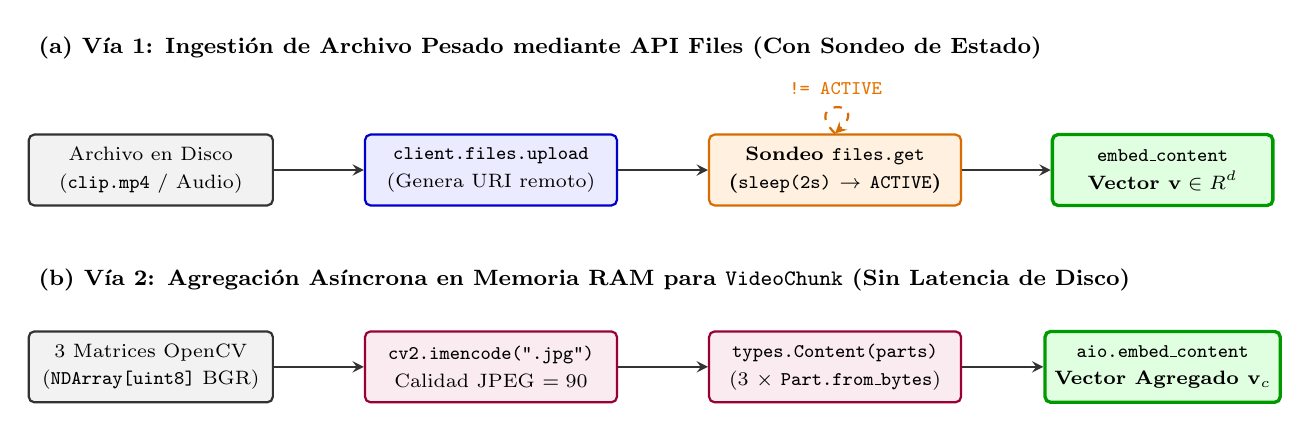
\begin{tikzpicture}[
    node distance=0.5cm and 0.65cm,
    box/.style={rectangle, draw=black!80, fill=gray!10, thick, minimum width=3.1cm, minimum height=0.90cm, align=center, font=\scriptsize, rounded corners=2pt},
    cloudbox/.style={rectangle, draw=blue!80!black, fill=blue!8, thick, minimum width=3.2cm, minimum height=0.90cm, align=center, font=\scriptsize, rounded corners=2pt},
    statebox/.style={rectangle, draw=orange!85!black, fill=orange!12, thick, minimum width=3.2cm, minimum height=0.90cm, align=center, font=\scriptsize\bfseries, rounded corners=2pt},
    membox/.style={rectangle, draw=purple!80!black, fill=purple!8, thick, minimum width=3.2cm, minimum height=0.90cm, align=center, font=\scriptsize, rounded corners=2pt},
    outbox/.style={rectangle, draw=green!60!black, fill=green!12, very thick, minimum width=2.8cm, minimum height=0.90cm, align=center, font=\scriptsize\bfseries, rounded corners=2pt},
    arrow/.style={-stealth, thick, draw=black!80}
]
% Vía A: API Files
\node[font=\bfseries\footnotesize, anchor=west] at (-7.9, 3.35) {(a) Vía 1: Ingestión de Archivo Pesado mediante API Files (Con Sondeo de Estado)};
\node[box] (f_disk) at (-6.35, 1.80) {Archivo en Disco\\[2pt](\texttt{clip.mp4} / Audio)};
\node[cloudbox] (f_up) at (-2.03, 1.80) {\texttt{client.files.upload}\\[2pt](Genera URI remoto)};
\node[statebox] (f_poll) at (2.34, 1.80) {Sondeo \texttt{files.get}\\[2pt](\texttt{sleep(2s)} $\to$ \texttt{ACTIVE})};
\node[outbox] (f_emb) at (6.50, 1.80) {\texttt{embed\_content}\\[2pt]Vector $\mathbf{v} \in \mathbb{R}^d$};

\draw[arrow] (f_disk) -- (f_up);
\draw[arrow] (f_up) -- (f_poll);
\draw[arrow] (f_poll) -- (f_emb);
\draw[arrow, dashed, orange!85!black] (f_poll.north) .. controls (1.9, 2.70) and (2.8, 2.70) .. node[above=1pt, font=\scriptsize\bfseries, text=orange!90!black] {\texttt{!= ACTIVE}} (f_poll.north);

% Vía B: Agregación en Memoria
\node[font=\bfseries\footnotesize, anchor=west] at (-7.9, 0.40) {(b) Vía 2: Agregación Asíncrona en Memoria RAM para \texttt{VideoChunk} (Sin Latencia de Disco)};
\node[box] (m_cv) at (-6.35, -0.70) {3 Matrices OpenCV\\[2pt](\texttt{NDArray[uint8]} BGR)};
\node[membox] (m_jpg) at (-2.03, -0.70) {\texttt{cv2.imencode(".jpg")}\\[2pt]Calidad JPEG $= 90$};
\node[membox] (m_part) at (2.34, -0.70) {\texttt{types.Content(parts)}\\[2pt](3 $\times$ \texttt{Part.from\_bytes})};
\node[outbox] (m_emb) at (6.50, -0.70) {\texttt{aio.embed\_content}\\[2pt]Vector Agregado $\mathbf{v}_c$};

\draw[arrow] (m_cv) -- (m_jpg);
\draw[arrow] (m_jpg) -- (m_part);
\draw[arrow] (m_part) -- (m_emb);
\end{tikzpicture}
\caption{Comparativa técnica de los dos flujos de ingestión en el SDK \texttt{google-genai}: (a) subida de archivos completos a la API Files con bucle de espera activa hasta alcanzar el estado \texttt{ACTIVE}, y (b) codificación JPEG en memoria de múltiples fotogramas empaquetados en un único objeto \texttt{types.Content} para llamadas asíncronas de baja latencia \cite{gemini_emb2_docs}.} %[cite: 3]
\label{fig:gemini_ingest_modes}
\end{figure}

Asimismo, para cerrar el ciclo de búsqueda cruzada y multimodal, el mismo componente vectorizador expone el método \texttt{embed\_query} (respaldado por \texttt{build\_query\_payload} y manteniendo \texttt{embed\_text} por retrocompatibilidad), capaz de empaquetar en un único contenedor \texttt{types.Content} cualquier combinación de consulta textual, ficheros \texttt{.txt}, imágenes de referencia codificadas a JPEG (\texttt{types.Part.from\_bytes}) y transcripciones de pistas de audio de entrada obtenidas con \texttt{transcribe\_query\_audios}. Al invocar \texttt{aio.models.embed\_content} en una sola llamada de red con idéntica configuración dimensional (\texttt{output\_dimensionality}) y normalización $L_2$, el sistema garantiza la compatibilidad algebraica exacta entre los fragmentos de vídeo indexados y las consultas multimodales del usuario \cite{gemini_emb2_docs}. %[cite: 3]

\subsubsection{Modelado Matemático de Cuotas Operativas (RPM, TPM y RPD) y Planificación de Capacidad}
\label{subsubsec:modelado_cuotas_capacidad}

Un aspecto crítico en el diseño de arquitecturas de ingeniería basadas en modelos fundacionales en la nube es la caracterización matemática de los límites de tasa (\textit{Rate Limits}) impuestos por el proveedor del servicio \cite{gemini_emb2_docs}. %[cite: 3]
En el entorno de experimentación y validación de Google AI Studio (capa gratuita o \textit{Free Tier}) para el modelo \texttt{gemini-embedding-2-preview}, la infraestructura impone simultáneamente tres umbrales restrictivos \cite{gemini_emb2_docs}: %[cite: 3]
\begin{itemize}
    \item \textbf{RPM (\textit{Requests Per Minute}):} Límite máximo de $\text{RPM}_{\max} = 100$ peticiones por minuto \cite{gemini_emb2_docs}. %[cite: 3]
    \item \textbf{TPM (\textit{Tokens Per Minute}):} Límite máximo de $\text{TPM}_{\max} = 30.000$ \textit{tokens} procesados por minuto \cite{gemini_emb2_docs}. %[cite: 3]
    \item \textbf{RPD (\textit{Requests Per Day}):} Límite máximo acumulado de $\text{RPD}_{\max} = 1.000$ peticiones por día \cite{gemini_emb2_docs}. %[cite: 3]
\end{itemize}

Un análisis superficial podría sugerir que el sistema es capaz de vectorizar $100$ fragmentos de vídeo (\texttt{VideoChunk}) por minuto atenidos al umbral de $\text{RPM}_{\max} = 100$. %[cite: 3]
Sin embargo, el modelado riguroso de la carga útil multimedia demuestra que el verdadero cuello de botella por minuto reside en el consumo de \textit{tokens} ($\text{TPM}_{\max}$) \cite{gemini_emb2_docs}. %[cite: 3]
Cada imagen o fotograma enviado a los modelos de la familia Gemini consume una tasa base de aproximadamente $T_{\text{img}} \approx 258\text{--}300$ \textit{tokens} \cite{gemini_emb2_docs}. %[cite: 3]
Dado que el algoritmo de selección por entropía extrae $N_{\text{frames}} = 3$ fotogramas clave por cada \texttt{VideoChunk}, el coste en \textit{tokens} de una única petición de fragmento asciende según la Ecuación~\eqref{eq:tokens_por_chunk} a: %[cite: 3]

\begin{equation}
T_{\text{chunk}} = N_{\text{frames}} \times T_{\text{img}} \approx 3 \times 300 = 900 \text{ tokens/chunk}
\label{eq:tokens_por_chunk}
\end{equation} %[cite: 3]

Si el orquestador enviase el máximo permitido de $100$ peticiones en un minuto, la demanda de caudal ascendería a $100 \times 900 = 90.000$ \textit{tokens}/minuto, triplicando el límite de $\text{TPM}_{\max} = 30.000$ y provocando el rechazo inmediato de las peticiones con código de error HTTP \texttt{429 (Too Many Requests)}. %[cite: 3]
En consecuencia, el caudal máximo efectivo sostenido ($\lambda_{\text{efectivo}}$) en fragmentos por minuto queda determinado según la Ecuación~\eqref{eq:caudal_efectivo_chunks} por el mínimo entre la restricción de peticiones y la restricción de \textit{tokens}: %[cite: 3]

\begin{equation}
\lambda_{\text{efectivo}} = \min\!\left(\text{RPM}_{\max}, \, \left\lfloor \frac{\text{TPM}_{\max}}{T_{\text{chunk}}} \right\rfloor\right) = \min\!\left(100, \, \left\lfloor \frac{30.000}{900} \right\rfloor\right) \approx 33 \text{ chunks/minuto}
\label{eq:caudal_efectivo_chunks}
\end{equation} %[cite: 3]

Esto restringe la velocidad de ingestión real a un rango de entre $30$ y $35$ fragmentos de vídeo por minuto, lo que significa que un vídeo de prueba que genere entre $100$ y $200$ \textit{chunks} requerirá entre $3$ y $6$ minutos de procesamiento continuo. %[cite: 3]

De forma análoga, el límite diario de $\text{RPD}_{\max} = 1.000$ peticiones acota la duración máxima de vídeo que puede indexarse en una jornada de experimentación. %[cite: 3]
Bajo una segmentación semántica adaptativa (\textit{Video-RAC}), un vídeo educativo o divulgativo promedio experimenta un cambio de plano cada $\bar{d}_{\text{plano}} \in [3, 7]$ segundos. %[cite: 3]
Asumiendo una media conservadora de $\bar{d}_{\text{plano}} = 5$ segundos por fragmento, cada minuto de metraje produce $C_{\text{min}} = 60 / 5 = 12$ \textit{chunks}/minuto, lo que arroja un límite teórico absoluto de duración diaria ($D_{\max}$) formulado en la Ecuación~\eqref{eq:duracion_maxima_diaria}: %[cite: 3]

\begin{equation}
D_{\max} = \frac{\text{RPD}_{\max}}{C_{\text{min}}} = \frac{1.000 \text{ chunks/día}}{12 \text{ chunks/minuto}} \approx 83,3 \text{ minutos/día}
\label{eq:duracion_maxima_diaria}
\end{equation} %[cite: 3]

Para evitar que el procesamiento accidental de un único archivo de larga duración agote el $100\%$ de la cuota diaria e impida realizar búsquedas o iteraciones de calibración durante el resto del día, la arquitectura de ingeniería implementa dos salvaguardas: acotar los vídeos de validación de la Prueba de Concepto a clips de entre \textbf{5 y 15 minutos} (que generan entre $100$ y $200$ \textit{chunks}, consumiendo apenas un $10\%\text{--}20\%$ del RPD), e incorporar en el orquestador un cortafuegos estático (\textit{fail-safe}) definido por la constante \texttt{MAX\_CHUNKS\_PER\_VIDEO = 800}. %[cite: 3]
Si tras la detección de bordes de plano con OpenCV el vídeo supera los $800$ fragmentos, el sistema aborta preventivamente lanzando la excepción \texttt{QuotaSafetyError} antes de extraer fotogramas ni consumir una sola petición de la API. %[cite: 3]

La Figura~\ref{fig:cuello_botella_tpm_rpd} esquematiza la interacción entre los tres umbrales de cuota y los mecanismos de protección implementados en el flujo de ingestión. %[cite: 3]

\begin{figure}[htbp]
\centering
\begin{tikzpicture}[
    node distance=0.5cm and 0.7cm,
    innode/.style={rectangle, draw=black!80, fill=gray!10, thick, minimum width=3.0cm, minimum height=1.2cm, align=center, font=\scriptsize, rounded corners=2pt},
    guardnode/.style={diamond, aspect=2.0, draw=red!80!black, fill=red!8, very thick, minimum width=2.8cm, minimum height=1.3cm, align=center, font=\scriptsize\bfseries},
    limitbox/.style={rectangle, draw=blue!80!black, fill=blue!8, thick, minimum width=4.0cm, minimum height=1.9cm, align=center, font=\scriptsize, rounded corners=3pt},
    abortbox/.style={rectangle, draw=red!80!black, fill=red!12, very thick, minimum width=3.2cm, minimum height=1.0cm, align=center, font=\scriptsize\bfseries, rounded corners=2pt},
    okbox/.style={rectangle, draw=green!60!black, fill=green!12, very thick, minimum width=4.0cm, minimum height=1.3cm, align=center, font=\scriptsize\bfseries, rounded corners=2pt},
    arrow/.style={-stealth, thick, draw=black!80}
]
\node[innode] (vid) at (-5.1, 0.0) {\textbf{Vídeo Segmentado}\\[2pt]$N$ \texttt{VideoChunks}\\($\sim 12$ chunks/min)};

\node[guardnode] (guard) at (-1.0, 0.0) {¿$N > 800$?\\(\texttt{MAX\_CHUNKS})};

\node[abortbox] (abort) at (-1.0, 2.1) {\texttt{QuotaSafetyError}\\[2pt]Aborta sin gastar API\\(Protege 1.000 RPD)};

\node[limitbox] (tpm) at (4.5, 0.0) {\textbf{Control de Caudal API}\\[2pt]
$\bullet$ $\text{RPM}_{\max} = 100$ pet/min\\[1pt]
$\bullet$ $\text{TPM}_{\max} = 30.000$ tok/min\\[1pt]
$\bullet$ Coste $\approx 900$ tok/chunk\\[2pt]
\textbf{Techo real: $\sim 33$ chunks/min}};

\node[okbox] (out) at (4.5, -2.35) {\textbf{Ingestión Controlada}\\[2pt]Clips 5-15 min (100-200 chunks)\\[1pt]Consumo: 10\%-20\% RPD};

\draw[arrow] (vid) -- (guard);
\draw[arrow, draw=red!80!black] (guard) -- node[right=3pt, font=\scriptsize\bfseries, text=red!80!black] {Sí} (abort);
\draw[arrow, draw=green!50!black] (guard) -- node[above=2pt, font=\scriptsize\bfseries, text=green!50!black] {No ($\le 800$)} (tpm);
\draw[arrow] (tpm) -- (out);
\end{tikzpicture}
\caption{Modelado de capacidad y cortafuegos de cuota para \texttt{gemini-embedding-2-preview}: la validación previa aborta ejecuciones que superen los $800$ fragmentos para proteger el límite diario (1.000 RPD), mientras que la densidad de $\sim 900$ \textit{tokens} por fragmento fija el caudal efectivo en $\sim 33$ \textit{chunks}/minuto bajo el techo de 30.000 TPM \cite{gemini_emb2_docs}.} %[cite: 3]
\label{fig:cuello_botella_tpm_rpd}
\end{figure}

\subsubsection{Ingeniería de Resiliencia: Control de Concurrencia, Ventana de \textit{Backoff} de 60 Segundos y Degradación Elegante}
\label{subsubsec:resiliencia_backoff_degradacion}

Dado que el procesamiento de vídeo combina operaciones intensivas de CPU (decodificación de fotogramas y cálculo de mapas gaussianos SSIM en OpenCV) con operaciones asíncronas de red (llamadas HTTP a la API de Gemini), la arquitectura de software debe evitar tanto el bloqueo del bucle de eventos como la saturación de los servidores remotos. %[cite: 3]

En primer lugar, las funciones síncronas bloqueantes de visión por computador (\texttt{detect\_shot\_boundaries} y \texttt{extract\_key\_frames}) se delegan a hilos secundarios mediante \texttt{asyncio.to\_thread}, liberando el hilo principal de Python para gestionar las conexiones de red. %[cite: 3]
En segundo lugar, la emisión paralela de tareas de vectorización en \texttt{asyncio.gather} se regula mediante un semáforo asíncrono (\texttt{asyncio.Semaphore(max\_concurrent\_requests)}) calibrado específicamente en \texttt{max\_concurrent\_requests = 3} (reducido respecto a un valor inicial de $5$) para impedir ráfagas instantáneas que desborden las cuotas por minuto. %[cite: 3]

Pese al uso del semáforo, dado que la latencia de respuesta de una petición individual es inferior a un segundo, tres corrutinas concurrentes pueden alcanzar el techo de $30.000$ \textit{tokens} antes de que se cumpla el minuto natural, recibiendo un error transitorio HTTP \texttt{429}. %[cite: 3]
Para absorber este fenómeno sin perder datos (así como fallos transitorios de servidor catalogados en el conjunto inmutable \texttt{\_RETRYABLE\_CODES = \{429, 500, 502, 503, 504\}} y errores de red \texttt{OSError}/\texttt{TimeoutError}), el método privado \texttt{\_embed} implementa un algoritmo de \textbf{reintento con espera exponencial (\textit{Exponential Backoff})}. %[cite: 3]

La calibración matemática de los parámetros de este \textit{backoff} resulta determinante: si se utilizase una espera base de $t_0 = 2,0\text{ s}$ con $R = 3$ reintentos, la suma de las pausas sería únicamente de $2 + 4 + 8 + 16 = 28\text{ s}$ (o $2+4+8 = 14\text{ s}$ en tres esperas), tiempo insuficiente para que Google reinicie la ventana deslizante de $60$ segundos del límite TPM. %[cite: 3]
Por el contrario, al incrementar los parámetros por defecto a un retardo base de \texttt{retry\_base\_delay} $= 4,0\text{ s}$ y un máximo de \texttt{max\_retries} $= 4$ reintentos, el tiempo de espera en el intento $k \in \{0, 1, 2, 3\}$ responde a $\Delta t_k = 4,0 \times 2^k$, generando una ventana acumulada calculada según la Ecuación~\eqref{eq:suma_backoff_60s}: %[cite: 3]

\begin{equation}
T_{\text{espera total}} = \sum_{k=0}^{3} t_0 \cdot 2^k = 4,0 \times (2^0 + 2^1 + 2^2 + 2^3) = 4 + 8 + 16 + 32 = 60 \text{ segundos}
\label{eq:suma_backoff_60s}
\end{equation} %[cite: 3]

La Figura~\ref{fig:backoff_ventana_60s} muestra cómo esta progresión geométrica cubre exactamente los $60$ segundos necesarios para garantizar la renovación de la cuota de \textit{tokens} por minuto antes de agotar el último intento. %[cite: 3]

\begin{figure}[htbp]
\centering
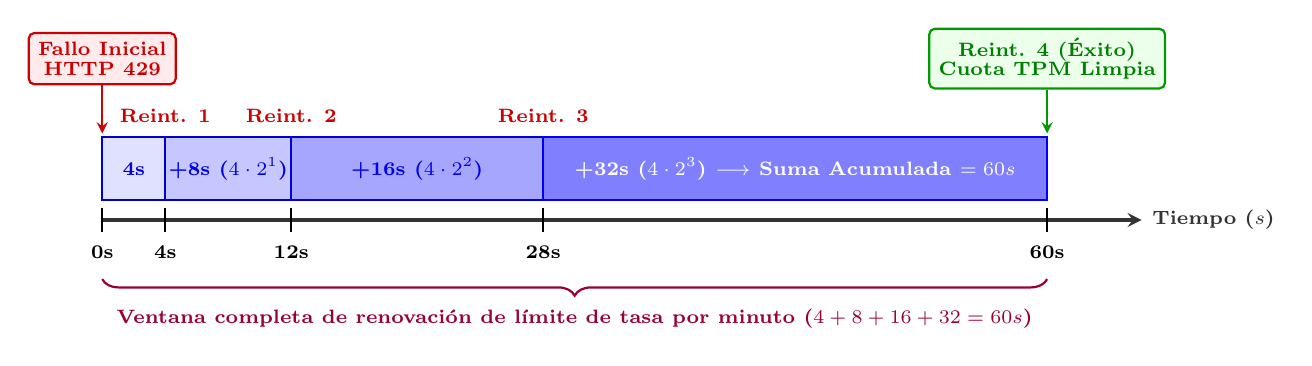
\begin{tikzpicture}
% Línea base de tiempo (0 a 60 segundos)
\draw[-stealth, very thick, black!80] (0,0) -- (13.2,0) node[right, font=\scriptsize\bfseries] {Tiempo ($s$)};

% Marcas de tiempo proporcionales (escala: 1 seg = 0.2 unidades -> 60s = 12.0 unidades)
\foreach \x/\t in {0/0s, 0.8/4s, 2.4/12s, 5.6/28s, 12.0/60s} {
    \draw[thick, black] (\x, 0.15) -- (\x, -0.15);
    \node[below, font=\scriptsize\bfseries] at (\x, -0.2) {\t};
}

% Bloques de espera exponencial
\draw[fill=blue!12, draw=blue!80!black, thick] (0, 0.25) rectangle (0.8, 1.05);
\node[font=\scriptsize\bfseries, blue!90!black] at (0.4, 0.65) {4s};

\draw[fill=blue!22, draw=blue!80!black, thick] (0.8, 0.25) rectangle (2.4, 1.05);
\node[font=\scriptsize\bfseries, blue!90!black] at (1.6, 0.65) {+8s ($4\cdot 2^1$)};

\draw[fill=blue!35, draw=blue!85!black, thick] (2.4, 0.25) rectangle (5.6, 1.05);
\node[font=\scriptsize\bfseries, blue!95!black] at (4.0, 0.65) {+16s ($4\cdot 2^2$)};

\draw[fill=blue!50, draw=blue!95!black, thick] (5.6, 0.25) rectangle (12.0, 1.05);
\node[font=\scriptsize\bfseries, white] at (8.8, 0.65) {+32s ($4\cdot 2^3$) $\longrightarrow$ Suma Acumulada $= 60\text{ s}$};

% Eventos de fallo e intento exitoso
\node[draw=red!80!black, fill=red!8, thick, rounded corners=2pt, font=\scriptsize\bfseries, text=red!80!black, align=center] (fail0) at (0.0, 2.05) {Fallo Inicial\\[-1pt]HTTP 429};
\draw[-stealth, thick, red!80!black] (fail0.south) -- (0.0, 1.10);

\node[above=2pt, font=\scriptsize\bfseries, text=red!80!black] at (0.8, 1.05) {Reint. 1};
\node[above=2pt, font=\scriptsize\bfseries, text=red!80!black] at (2.4, 1.05) {Reint. 2};
\node[above=2pt, font=\scriptsize\bfseries, text=red!80!black] at (5.6, 1.05) {Reint. 3};

\node[draw=green!60!black, fill=green!8, thick, rounded corners=2pt, font=\scriptsize\bfseries, text=green!50!black, align=center] (succ) at (12.0, 2.05) {Reint. 4 (Éxito)\\[-1pt]Cuota TPM Limpia};
\draw[-stealth, thick, green!60!black] (succ.south) -- (12.0, 1.10);

% Llave inferior de ventana de 1 minuto
\draw[decorate, decoration={brace, amplitude=6pt, mirror}, thick, purple!80!black] (0, -0.75) -- (12.0, -0.75) node[midway, below=7pt, font=\scriptsize\bfseries, purple!80!black] {Ventana completa de renovación de límite de tasa por minuto ($4 + 8 + 16 + 32 = 60\text{ s}$)};
\end{tikzpicture}
\caption{Cronograma temporal del algoritmo de \textit{Exponential Backoff} calibrado (\texttt{retry\_base\_delay = 4.0}, \texttt{max\_retries = 4}): la suma geométrica de las cuatro esperas alcanza exactamente $60$ segundos, permitiendo superar bloqueos completos de la ventana de 30.000 TPM sin abortar la vectorización del fragmento.} %[cite: 3]
\label{fig:backoff_ventana_60s}
\end{figure}

Adicionalmente, el diseño incorpora dos mecanismos de \textbf{Degradación Elegante (\textit{Graceful Degradation})} en distintas capas del sistema para garantizar una tolerancia a fallos de nivel industrial: %[cite: 3]
\begin{enumerate}
    \item \textbf{Aislamiento de fallos parciales en la fase de ingestión (\texttt{return\_exceptions=True}):} Si tras agotar los $60$ segundos de reintentos un fragmento puntual sigue fallando (lanzando \texttt{VectorizationError}), la invocación \texttt{asyncio.gather(* tasks, return\_exceptions=True)} evita que se cancele el lote completo. %[cite: 3]
    El orquestador captura la excepción de ese único \textit{chunk}, la documenta en \texttt{execution.log} mediante el auditor (\texttt{RunAuditor}) y conserva intactos todos los demás fragmentos vectorizados del vídeo. %[cite: 3]
    \item \textbf{Respaldo vectorial ante caídas \texttt{503 UNAVAILABLE} en la segunda etapa de reordenación visual:} Durante la fase de búsqueda y refinamiento con modelos ligeros de visión-lenguaje (como \texttt{gemini-3.5-flash-lite}), los servidores de Google pueden experimentar picos temporales de demanda devolviendo el error \texttt{503 UNAVAILABLE ("This model is currently experiencing high demand")}. %[cite: 3]
    Cuando esto ocurre y se agotan los reintentos del verificador secundario, el sistema no colapsa ni devuelve un error al usuario: intercepta la indisponibilidad, emite un aviso informando que la reordenación visual no está disponible temporalmente y \textbf{conserva automáticamente el orden vectorial original devuelto por Qdrant} en la primera etapa. %[cite: 3]
\end{enumerate}

La Figura~\ref{fig:degradacion_elegante_503} representa este flujo de continuidad operativa y degradación elegante en ambas fases de la arquitectura. %[cite: 3]

\begin{figure}[htbp]
\centering
\begin{tikzpicture}[
    node distance=0.5cm and 0.65cm,
    proc/.style={rectangle, draw=blue!80!black, fill=blue!8, thick, minimum width=3.1cm, minimum height=1.1cm, align=center, font=\scriptsize, rounded corners=2pt},
    dec/.style={diamond, aspect=1.9, draw=orange!85!black, fill=orange!10, thick, minimum width=2.3cm, minimum height=1.2cm, align=center, font=\scriptsize\bfseries},
    warn/.style={rectangle, draw=purple!80!black, fill=purple!10, thick, minimum width=3.2cm, minimum height=1.2cm, align=center, font=\scriptsize, rounded corners=2pt},
    ok/.style={rectangle, draw=green!60!black, fill=green!12, very thick, minimum width=3.2cm, minimum height=1.2cm, align=center, font=\scriptsize, rounded corners=2pt},
    arrow/.style={-stealth, thick, draw=black!80}
]
\node[proc] (qdrant) at (-6.25, 0.0) {\textbf{1.ª Etapa: Qdrant}\\[2pt]Recupera Top-$K$ por\\Similitud Coseno};

\node[proc] (rerank) at (-1.95, 0.0) {\textbf{2.ª Etapa: Verificador}\\[2pt]{\scriptsize \texttt{gemini-3.5-flash-lite}}\\[1pt]+ Backoff Exponencial};

\node[dec] (status) at (1.90, 0.0) {¿HTTP 503\\Persiste?};

\node[warn] (fallback) at (1.90, 2.1) {\textbf{Degradación Elegante}\\[2pt]Log: \textit{Fallo 503 VLM}\\[1pt]Omite filtro secundario};

\node[ok] (out_rerank) at (6.20, 0.0) {\textbf{Resultados Top-}$K$\\[2pt]Reordenados por VLM\\(Máxima precisión)};

\node[ok, draw=teal!80!black, fill=teal!12] (out_vec) at (6.20, 2.1) {\textbf{Resultados Top-}$K$\\[2pt]Orden Vectorial Original\\(Preserva ranking Qdrant)};

\draw[arrow] (qdrant) -- (rerank);
\draw[arrow] (rerank) -- (status);
\draw[arrow, draw=red!80!black] (status) -- node[right=3pt, font=\scriptsize\bfseries, text=red!80!black] {Sí (503)} (fallback);
\draw[arrow, draw=green!50!black] (status) -- node[above=2pt, font=\scriptsize\bfseries, text=green!50!black] {No (200 OK)} (out_rerank);
\draw[arrow, draw=purple!80!black] (fallback) -- (out_vec);
\end{tikzpicture}
\caption{Arquitectura de Degradación Elegante (\textit{Graceful Degradation}) durante la búsqueda: si los servidores del modelo secundario (\texttt{gemini-3.5-flash-lite}) sufren picos de saturación (\texttt{503 UNAVAILABLE}) tras agotar los reintentos, el sistema conmuta limpiamente al orden de similitud vectorial calculado por Qdrant con \textit{Gemini Embedding 2}.} %[cite: 3]
\label{fig:degradacion_elegante_503}
\end{figure}

El Cuadro~\ref{tab:parametros_gemini_vectorizer} sintetiza los parámetros definitivos de ingeniería calibrados en el sistema para maximizar la fiabilidad bajo las restricciones operativas de la API de Google. %[cite: 3]

\begin{table}[htbp]
\centering
\small
\caption{Parámetros técnicos calibrados en los módulos de vectorización y orquestación para operar con \texttt{gemini-embedding-2-preview} sin colapsos de cuota \cite{gemini_emb2_docs}.} %[cite: 3]
\label{tab:parametros_gemini_vectorizer}
\begin{tabularx}{\linewidth}{p{4.2cm}p{3.2cm}p{2.6cm}X}
\toprule
\textbf{Parámetro} & \textbf{Módulo} & \textbf{Valor} & \textbf{Justificación Técnica / MLOps} \\
\midrule
\texttt{model} & \texttt{gemini\_vectorizer.py} & \texttt{gemini-embedding-2} & Modelo omnimodal nativo (espacio compartido) \\
\texttt{output\_dimensionality} & \texttt{gemini\_vectorizer.py} & $3.072$, $1.536$ o $768$ & MRL con normalización $L_2$ (\texttt{truncate\_and\_normalize\_mrl}) \\
\texttt{jpeg\_quality} & \texttt{gemini\_vectorizer.py} & $90$ (escala $1\text{-}100$) & Alta fidelidad visual en RAM sin artefactos \\
\texttt{max\_concurrent\_requests} & \texttt{pipeline.py} & $3$ (reducido de $5$) & Limita peticiones concurrentes en semáforo \\
\texttt{retry\_base\_delay} & \texttt{gemini\_vectorizer.py} & $4,0\text{ s}$ (antes $2,0\text{ s}$) & Base geométrica para cubrir ventana TPM \\
\texttt{max\_retries} & \texttt{gemini\_vectorizer.py} & $4$ (antes $3$) & Suma $4+8+16+32 = 60\text{ s}$ ante error HTTP \\
\texttt{MAX\_CHUNKS\_PER\_VIDEO} & \texttt{pipeline.py} & $800$ fragmentos & Cortafuegos \texttt{QuotaSafetyError} (protege RPD) \\
\bottomrule
\end{tabularx}
\end{table}